%%% This is an example file for the Auburn University style options
%%%       aums.sty (Masters Thesis)
%%%       auphd.sty (Ph.D. Dissertation)
%%%       auhonors.sty (Honors Scholar)

%%%To use it, please edit the necessary options, title, author, date, year, keywords, advisor, professor, etc. 

\documentclass[12pt]{report}
\usepackage{aums}       % For Master's papers
\usepackage{ulem}       % underlining on style-page; see \normalem below
\usepackage{url}
\usepackage{tikz}
\usepackage{pgf}
\usepackage{graphicx}
\usepackage{array}
%%%%%Format rules: Normal margins are 1 in. If you need to print with 1.5in margins, uncomment the line below
%\oddsidemargin0.5in \textwidth6in

%% If you do not need a List of Abbreviations, then comment out the lines below and the \printnomenclature line.
%%for List of Abbreviations information:  (see http://www.mackichan.com/TECHTALK/509.htm  )
\usepackage[intoc]{nomencl}
\renewcommand{\nomname}{List of Abbreviations}   	       
\makenomenclature 
%% don't forget to run:   makeindex ausample.nlo -s nomencl.ist -o ausample.nls

% This is so I can highlight things to get my attention when todoinepackage{color}
\usepackage{soul}
\newcommand{\todo}[1]{\hl{TODO: #1}}

% May want theorems numbered by chapter
\newtheorem{theorem}{Theorem}[chapter]

% Put the title, author, and date in. 
\title{Evaluating the Digital Fault Coverage for a Mixed-Signal Built-In Self Test}
\author{Michael Alexander Lusco} 
\date{May 10, 2011} %date of graduation
\copyrightyear{2011} %copyright year

\keywords{Built-In Self Test, Mixed-Signal, Testing}

% Put the Thesis Adviser here. 
\adviser{Charles Stroud}


% Put the committee here (including the adviser), one \professor for each. 
% The advisor must be first, and the dean of the graduate school must be last.
\professor{Charles Stroud, Chair, Professor of Electrical and Computer Engineering}

\professor{Foster Dai, Co-Chair, Professor of Electrical and Computer Engineering}

\professor{Vashani Agrawal, Professor of Eletrical and Computer Engineering}

\professor{Victor Nelson, Professor of Eletrical and Computer Engineering}

\begin{document}

\begin{romanpages}      % roman-numbered pages 

\TitlePage 

\begin{abstract}
This thesis focuses on a digital Built-in Self-Test (BIST)\nomenclature{BIST}{Built-in Self-Test} approach to perform specification-oriented testing of the analog portion of a mixed-signal system.  The BIST utilizes a Direct Digital Synthesizer (DDS)\nomenclature{DDS}{Direct Digital Synthesizer} based test pattern generator (TPG)\nomenclature{TPG}{Test Pattern Generator} and a multiplier-accumulate (MAC)\nomenclature{MAC}{Multiplier-Accumulator} based output response analyzer (ORA)\nomenclature{ORA}{Output Response Analyzer} to stimulate and analyze the analog devices under test.  This approach uses the digital-to-analog convertor (DAC)\nomenclature{DAC}{Digital-to-Analog Convertor} and the analog-to-digital convertor (ADC)\nomenclature{ADC}{Analog-to-Digital Convertor}, which typically already exist in a mixed signal circuits, to connect the digital BIST circuitry to the analog device(s) under test (DUT)\nomenclature{DUT}{Device Under Test}.

Previous work has improved and analyzed the capabilities and effectiveness of using this BIST approach to test analog circuitry; however, little work has been done to determine the fault coverage of the digital BIST cicuitry iteself.  Traditionally additional test circuitry such as scan chains would be added to the BIST circuitry to provide adequate fault coverage of digital circuitry.  WHile ensuring that the digital circuitry is throughly tested and functioning properly, this scan chain circuitry incures a potentially high area overhead and performance penalty.  This thesis focues on using the existing BIST circuitry to test itself by utilizing a dedicated gitial loopback path.  A set of test procedures is proposed and analyzed which can be used to determine a set of functional tests which provide a high effective fault coverage of the digital porition of the BIST.  TO determine the effectiveness of these procedures, the mixed-signal BIST circuit is simulated and single stuck-at gate-level fault coverage results are determined and presented.  Finally several improvements to the dedicated loopback path are proposed and simulated to analyze possible ways to improve the fault coverage of the BIST with minimal area and performance impact.
\end{abstract}

\begin{acknowledgments}
Put text of the acknowledgments here.
\end{acknowledgments}

\tableofcontents
\listoffigures
\listoftables

\printnomenclature[0.5in] %used for the List of Abbreviations
\end{romanpages}        % All done with roman-numbered pages


\normalem       % Make italics the default for \em


\chapter{Introduction}  % Use \\ for long titles 

The testing of embedded systems is a large field with many different approaches and techniques.  Some techniques work most effectively for digital systems and others for analog systems.  One approach is a hybrid and is used to test a mixed-signal system -- a system with both digital and analog circuitry.  Mixed systems typically require the use of multiple testing techniques from both the digital and analog domains to be fully tested.  In this chapter a short introduction to testing and relevant testing techniques for digital, analog, and mixed-signal systems is given so that the reader can develop a foundation for understanding the mixed-signal testing approach studied in this thesis. 

\section{Why Test Circuits}
\label{sct:whytest}
According to Stroud\cite{stroud} there are three phases of a product where testing is of critical importance: the design phase, manufacturing phase, and the system operation phase.  Each phase of the product's life cycle uses testing to achieve different goals.  During the design phase of the product life cycle, the goal is to focus on finding and eliminating design errors.  During manufacturing the goal changes and is focused on eliminating manufacturer defects, and finally the operation phase is focused on ensuring error-free operation.  All of these different testing goals work to improve the device by reducing costs, improving relability, etc.  

\section{The Basics of Testing}
\label{sct:basictesting}

The basics of testing a circuit are similar during all phases of a product's life-cycle:
\begin{itemize}
\item Generate a set of input stimuli or vectors
\item Apply those vectors to the DUT
\item Compare the output of the DUT to the expected output for each input value
\item Note any discrepancies as indication that there is an error in the device (a fault)
\end{itemize}
In reality it is often more difficult to test circuits than this basic process makes it appear.  One way to ease this difficulty is by using design for testability (DFT)\nomenclature{DFT}{Design For Testability} techniques to increase the observability and controllability of a device during the design process\cite{stroud}.  Stroud defines observability and controllability in \cite{stroud} as the following:
\begin{quote}
``Controllability is the ease with which we can control a fault site and observability is the ease with which we can observe a fault site.\cite{stroud}''
\end{quote}
Ultimately these properties determine the complexity of testing a circuit.  As chips grow it becomes increasingly challenging to maintain an acceptable level of controllability and observability.  According to \cite{zorian}: 
\begin{quote}
``The growth rate in integrated circuit (IC)\nomenclature{IC}{Integrated Circuit} transistor count is far higher than the rate for IC pins and steadily reduces the accessibility of transistors from chip pins -- a big problem for IC test.\cite{zorian}''
\end{quote}
Large, modern circuits can contain billions of transistors and comparatively few IO pins\cite{zorian}.  Without careful design considerations these properties can negatively affect the testability of a device\cite{stroud}.

There are many different methods to physically testing a device.  Each method varies in its requirements and has its own unique set of challenges, costs, and advantages.  One traditional method of testing uses automatic testing equipment.  Automatic test equipment is commonly used during manufacturing to verify chips are manufactured without defects\cite{zorian}.  Unfortunately as the complexity and speed of IC's has increased, automatic testing equipment has struggled to maintain an acceptable test coverage of performance-related defects\cite{zorian}.  To test these more complex circuits requires more advanced and higher speed automatic test equipment with additional IO capabilities\cite{zorian}.  \cite{zorian} examines the cost of high-end automatic test equipment and finds they may become cost prohibitive for complex circuits.  \cite{itrs} estimates that without the inclusion of alternative testing approaches ``tester costs will reach up to \$20 million dollars in 2010''. One such alternative to more expensive testing equipment is Built-in Self-Test. BIST describes the technique of designing a device to test itself\cite{stroud} and can complement or eliminate the need for automatic test equipment\cite{zorian}.

\section{Built-In Self-Test}
\cite{stroud} defines BIST as a circuit which can test itself and determine whether it is ``good'' or ``faulty.''  In essence this entails designing the circuit to perform all of the steps in section \ref{sct:basictesting} on itself.  \cite{stroud} continues by outlining the basics of a BIST architecture.  This simple architecture consists of several major components including a Test Pattern Generator (TPG)\nomenclature{TPG}{Test Pattern Generator} which generates the input stimuli necessary to test the circuit and an Output Response Analyzer or ORA\nomenclature{ORA}{Output Response Analyzer} which compares the output of the circuit to the expected output for a given input value.  Additionally there is circuitry which isolates the DUT during testing as well as circuitry which controls the test during execution (Test Controller)\cite{stroud}.

BIST has many advantages and disadvantages when compared to other techniques.  \cite{stroud} quantifies these advantages and disadvantages in Table \ref{tbl:advantages}. 
\begin{table}
	\caption{Advantages and Disadvantages of BIST\cite{stroud}}
	\begin{center}
	\begin{tabular}{|l|l|}
		\hline
		\multicolumn{1}{|c|}{{\bf Advantages}} & \multicolumn{1}{|c|}{{\bf Disadvantages}} \\ \hline
		Vertical testability (wafter to system) & Area overhead \\ \hline
		High Diagnostic resolution & Performance penalties \\ \hline
		At-speed testing & Additional design time \& effort \\ \hline
		Reduced need for automatic test equipment & Additional risk to project \\ \hline
		Reduced test development time \& effort & \\ \hline
		More economical burn-in testing & \\ \hline
		Reduced manufacturing test time \& cost & \\ \hline
		Reduced time-to-market & \\ \hline
	\end{tabular}
	\end{center}
	\label{tbl:advantages}
\end{table}
In addition \cite{ungar} performs a detailed economic analysis of including BIST in circuitry. \cite{ungar} concludes that:
\begin{quote}
``As the product develops from the IC to system level and its complexity increases, so does the complexity of successfully identifying a failure's root cause.  So it makes economic sense for system owners and perhaps system producers to implement BIST.\cite{ungar}''
\end{quote}
The advantages of BIST and its ability to reduce test time and cost make it an excellent choice for testing devices\cite{zorian}.

\subsection{Digital Systems and Faults}
\label{sct:digitalsystems}
Faults in a system are characterized by a fault model.  A common model used for digital systems (systems functioning at discrete `1' and `0' logic values) is the gate-level stuck-at fault model\cite{stroud}.  According to \cite{stroud}, the stuck-at fault model allows for faults at the input or output of a digital logic gate.  These faults can cause the input or output to be stuck-at a logic value `0' or `1' regardless of which value is applied or expected.  

Figure \ref{fig:andtruth} provides a truth table listing the faulty and fault-free output of an AND gate with its `A' input stuck-at `1'.  The `X' notation is used to indicate the location of the fault and the `SA1' (or `SA0') designates rather the fault is a stuck-at `1' or stuck-at '0'\cite{stroud}.  The truth table given in Figure \ref{fig:andtruth} shows how a single fault can change the behavior of a gate often having a major impact on the overall behavior of the circuit.
\begin{figure}[b!]
	\begin{center}
	\begin{minipage}[l]{.45\textwidth}
		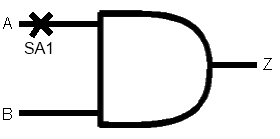
\includegraphics[scale=.7]{images/and-gate}
	\end{minipage}
	\begin{minipage}[r]{.45\textwidth}
		\begin{tabular}{|l|l|l|}
			\hline
			Inputs & Fault Free & Faulty \\
			(AB) & Output (Z) & Output (Z) \\ \hline
			0 0 & 0 & 0 \\ \hline
			0 1 & 0 & 1 \\ \hline
			1 0 & 0 & 0 \\ \hline
			1 1 & 1 & 1 \\ \hline
		\end{tabular}
	\end{minipage}
	\end{center}
	\caption{AND gate with input A stuck at 1}
	\label{fig:andtruth}
\end{figure}
Since digital circuits will always produce the same outputs for a given set of inputs, any difference between the expected and actual output can be exploited to determine if a circuit is functioning correctly\cite{stroud}.  Each clock cycle an input vector is applied and the output is compared with the expected output.  If any output does not match the expected output then the chip is considered faulty and discarded.  Unfortunately the storage required to hold each input and expected output vector can be significant for large or complex chips and while feasible for costly automatic test equipment, it is often impossible due to area considerations when using a BIST approach\cite{faultdiagnosis}.

When using BIST the input vectors are often generated by the TPG circuitry determinstically, algorithmically, or pseudo-randomly (among other methods)\cite{stroud}.  This keeps the size of the BIST to a minimum and removes the need for a large memory or other means of storing every input vector.  Likewise it is impratical to store every expected output pattern and compare it to the actual output each clock cycle.  To minimize storage requirements a signature is often used used to compress the output of the circuit into a single vector.  Instead of comparing each output at the end of each clock cycle, the signature is generated during the test and compared to the expected signature at the end of a test\cite{stroud}\cite{faultdiagnosis}.  A signature can be generated in a number of different ways and may be as simple as a counter counting the number of 1's or 0's which occur in the output, 1's or 0's counting, or as complex as using a large Multiple Input Signature Register\nomenclature{MISR}{Multiple Input Signature Register}\cite{stroud}.  The most appropriate signature generation method is dependent on the requirements and output of the design and can significantly impact the effectiveness of a BIST approach.  If a method is used which does not produce a suitably unique signature then faulty circuits can escape detection\cite{stroud}\cite{faultdiagnosis}.  The use of an expected signature to compress the circuit output allows for a significant reduction in storage cost as in most cases only a single comparison needs to be performed to verify the circuit\cite{faultdiagnosis}.

Returning to the example in Figure \ref{fig:andtruth}, a simple BIST can be constructed to test the AND gate.  In Figure \ref{fig:andbist} a 2-bit counter is used as the TPG to generate all of the inputs patterns possible for a two input AND gate: ``00'', ``01'', ``10'', and ``11''.  Also in the figure the output of the AND gate is connected to the \textit{Enable} of an additional 2-bit counter to count each `1' and produce a signature.  The fault-free signature for this circuit is ``01'' since a normally operating AND gate should only produce a single logic `1' when both its inputs are logic `1'.  If any input is stuck-at `1' then it will produce at least one additional `1'; if any input is stuck-at `0' it will never produce a logic `1'.  These two conditions will produce invalid signatures.  During execute of the BIST sequence, the TPG counts from ``00'' to ``11'' and the 1's counter will increment for each `1' occurring at the output of the gate.  At the end of the sequence, if the value in the 1's counter is not ``01'' then the gate is faulty.  This example is greatly simplified and is missing required circuitry to start and stop the BIST as well as a method to isolate the inputs of the gate; however, it does demonstrate the general principal behind using BIST to test a digital circuit.

\begin{figure}
	\begin{center}
		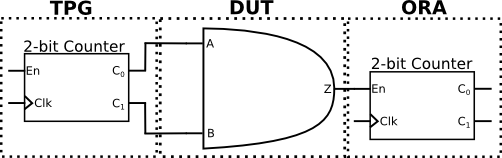
\includegraphics[scale=1]{images/and-bist}
	\end{center}
	\caption{BIST for an AND Gate}
	\label{fig:andbist}
\end{figure}

\subsection{Analog Systems and Faults}
\label{sct:AnalogFaults}

Analog systems function differently than digital systems.  Unlike a digital system which only has two discrete values, analog systems are continuous waveforms with multiple levels and voltages\cite{syschip}.  In addition to the complexities of analog waveforms, analog components operate within a range of acceptable values\cite{syschip}.  This difference makes testing analog components for defects (defect-oriented testing) significantly more challenging and requires a more complex fault model.  In analog components faults are classified as either parametric (soft-faults) or catastrophic (hard-faults)\cite{analogfaults}.  Parametric faults are those which affect the performance of a specific component causing it to operate outside of its expected tolerance range, for example a resistor which has a lower than expected resistance.  In constrast catastrophic faults are those which cause a component to fail, such as resistor which is no longer conductive and appears as an open circuit\cite{analogfaults}.  The simulation of these different faults requires complicated and time consuming methods such as Monte Carlo analysis to determine different component values which allow fault-free circuit operation\cite{syschip}.  Compounding these issues is the fact that analog components
\begin{quote}
``function collectively to perform the overall functionality of a given circuit and, as a result cannot always be treated as a collection of individual components\cite{syschip}.''
\end{quote}
and consequently are difficult to isolate for effective defect-oriented testing\cite{analogmixedtest}.  Furthermore any circuitry added into an analog circuit may potentially interfere and change the operating range or output of that circuit\cite{syschip}.  This potential interferance requires that any analog testing circuitry be carefully simulated and verified to ensure it does not negatively affect the overal circuit performance.  An example of a defected-oriented approach, oscillation testing is a testing approach which reconfigures the analog CUT so that it oscillates; this oscillation frequency is then measured and compared to an expected frequency.  If the measured frequency falls outside the expected range, the circuit is considered faulty\cite{analogosc}.  This method has been shown to be effective for the detection of catastrophic faults and some parametric faults; however, it can require a significant amount of planning and design effort as it may significantly impact the analog circuitry\cite{analogosc}\cite{syschip}.

A simpler (and preferred\cite{syschip}) method for testing analog components is via functional testing. \cite{milor} defines functional tests as: 
\begin{quote}
``... those which measure a circuit's dynamic behavior ...\cite{milor}''
\end{quote}
Functional or specification testing is achieved by performing a set of tests to determine if a system is operating correctly as defined by its specifications.  This approach is used to test the entire analog system collectively instead of attempting to understand the implications of specific faulty components\cite{analogmixedtest}.  Specification testing may include the testing of important analog characteristics such as frequency response, linearity, and signal-to-noise ratio (SNR)\nomenclature{SNR}{Signal-to-Noise Ratio}\cite{syschip}; however, the characteristics which are important  to test will vary between designs.  To adequately test most analog components, multiple measurements of several different characteristics must be taken as a single characteristic is usually not sufficent to ensure fault-free operation\cite{analogmixedtest}.  This process may require extra development time as test procedures must be developed to test each characteristic and additional time is required to perform each test\cite{analogmixedtest}.

\subsection{Mixed Signal Testing}
\label{sct:MixedSignal}
In a mixed-signal environment both digital and analog systems coexist and interact.  Due to the previously discussed differences in testing analog and digital systems, the testing of the analog and digital sub-systems is generally developed seperately and performed using using different test procedures and approaches\cite{analogmixedtest}.  Ideally a designer would like to limit any duplicate work and take advantage of a BIST approach which can be used to test both the analog and digital sub-systems.

\cite{stroud} defines a BIST approach to testing mixed-signal systems shown in Figure \ref{fig:mixedbist1}.  This BIST uses a digital BIST approach to functionally test the analog sub-system by measuring certain analog characteristics which can be used ensure that the circuit is operating within its specifications.  This architecture is largely digital and thus can be integrated into the digital circuitry already in the system with minimal analog overhead.  This prevents excessive interference with the analog circuitry, excluding multiplexors which faciltate the sending and retrieving of test values to and from the analog sub-system\cite{stroud}.  To test the analog circuitry, the BIST uses the existing Digital to Analog Converter (DAC)\nomenclature{DAC}{Digital to Analog Converter} to convert digitally generated test patterns from the TPG to analog signals and the existing Analog to Digital Converter (ADC)\nomenclature{ADC}{Analog to Digital Converter} to convert the analog response back into the digital domain for analysis by the ORA\cite{stroud}.
\begin{figure}
	\begin{center}
		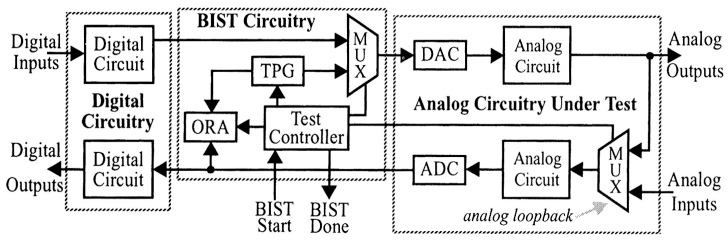
\includegraphics[scale=1]{images/mixed-bist-architecture}
	\end{center}
	\caption{BIST approach for mixed-signal systems\cite{stroud}}
	\label{fig:mixedbist1}
\end{figure}

Figure \ref{fig:mixedbist1} shows a basic version of this mixed-signal BIST approach using two multiplexors.  In this case one multiplexor is placed before the DAC to select between the BIST patterns and the system circuitry and a second multiplexor is positioned at the input of the analog system to select between the system level inputs and the analog outputs.  These two multiplexors form a loop allowing the generated TPG pattern to be converted into an analog signal and propogate through any analog circuitry before being routed back through the analog inputs to the DAC for analysis by the ORA.  While this implementation does allow testing of all analog components, it does not allow a high level of diagnostic resolution\cite{syschip}.  To obtain a higher diagnostic resolution, additional multiplexors can be added to further partition the system. Figure \ref{fig:mixedbist_paths} shows an example of an implementation with three seperate multiplexed or loopback paths to facilitate a higher level of diagnostic resolution.  In Figure \ref{fig:mixedbist_paths} the shortest loop, the short dashed path, is a digital only path (digital loopback path) which can be used to test that the digital BIST is fault free.  The next loopback path, the dashed path, connects the output of the DAC to the ADC bypassing any of the analog circuitry (from here on referred to as the bypass path).  This allows the verification of the ADC and DAC separately from the analog circuit.  The final path is the analog test path, the dotted path, and is similar to the path in Figure \ref{fig:mixedbist1} in that it is responsible for testing the analog circuitry.  There is no limit to the number of multiplexors that can be added to the system other than the increase in area overhead\cite{syschip}.  Additional multiplexors could be added to the example in Figure \ref{fig:mixedbist_paths} to further partition the analog circuitry and resolve faulty behavior to a specific portion of the analog cut.
\begin{figure}
	\begin{center}
		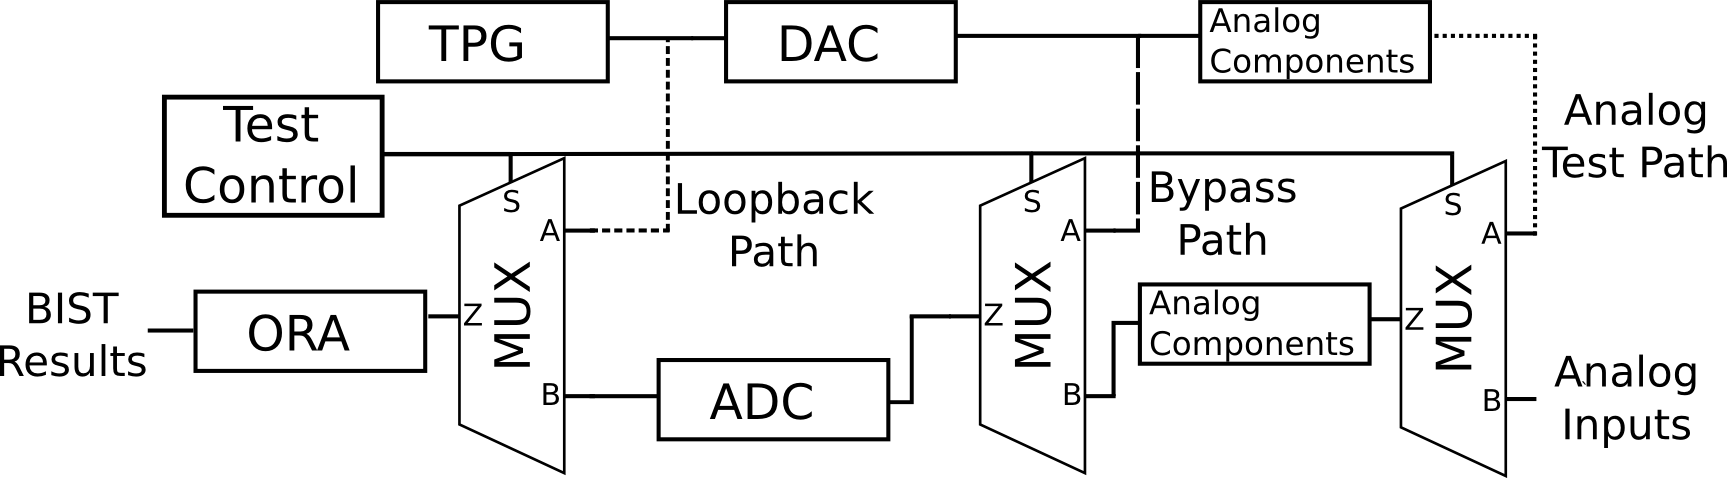
\includegraphics[scale=1]{images/mixedbist-paths}
	\end{center}
	\caption{Mixed-Signal BIST with multiple loopback paths}
	\label{fig:mixedbist_paths}
\end{figure}

In Figure \ref{fig:mixedbist_paths} the digital loopback path is of particular importance.  \cite{stroud-analog} has shown that a digital loopback path is highly advantageous when testing the digital portion of the BIST circuitry.  In a digital only environment the BIST produces exactly one output for a given set of inputs; however, without the digital loopback path the TPG outputs are not directly observable.  To observe the outputs of the TPG requires conversion via the DAC and reconversion via the ADC.  This will cause variations in the expected results due to the inherent variations which occur in analog signals and circuits.   To account for these variations, a range of acceptable values must be considered instead of an exact signature\cite{stroud-analog}.  

Figure \ref{fig:analog-faultcvg}
\begin{figure}
	\begin{center}
		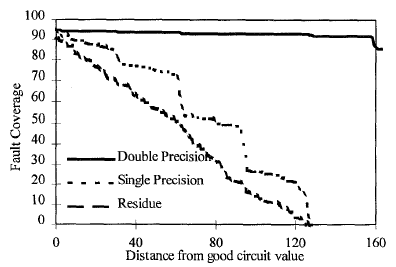
\includegraphics[scale=.6]{images/analog-fault-coverage}
	\end{center}
	\caption{Fault Coverage v. Acceptable Value Range\cite{stroud-analog}}
	\label{fig:analog-faultcvg}
\end{figure}
shows a comparison of the maximum achievable digital fault coverage versus the allowed distance away from the expected good signature for different ORA designs.  In the figure, three different 8-bit ORA accumulator designs are considered  (ORA design is discussed in more detail in the next chapter).   Figure \ref{fig:analog-faultcvg} shows that regardless of design a (in some cases significant) reduction in the maximum achievable fault coverage is to be expected when a range of good values is considered instead of an exact signature.  Thus the only way to achieve the maximum fault coverage is to not use a range of acceptable values and perform a digital only test.  This requires the digital loopback path\cite{stroud-analog}.  Performing a digital only test separates the digital and analog systems when testing.  This allows for the usage of tools and techniques which target digital components separately from those used to generate the analog functional tests on the analog sub-system\cite{stroud-analog}.  When the three loopback paths shown in Figure \ref{fig:mixedbist_paths} are present, the test procedure should be performed first over the digital loopback path to verify the digital BIST, then using the bypass path to verify that the ADC and DAC path are functioning correctly, and finally over the entire circuit to verify the analog DUT\cite{syschip}\cite{stroud-analog}.

Though this technique still requires the separate testing of the analog and digital circuitry, it is an improvement over the previously discussed method since the same BIST circuitry can be used to test both the digital and analog circuitry\cite{stroud}.  This limits the amount of work that must be duplicated to the determination of which tests to be run and the expected values.  Furthermore the basic procedure for testing the analog and digital circuits is the same (the only differences being which loopback path is selected and the actual test being performed) which will limit the differences between test sessions.

\section{Summary}
In the previous chapter a highlevel look at both digital and analog systems has been given as well as the challenges of testing these systems for faults.  The concept of BIST has been presented along with its advantages and a simple BIST architecture.  In addition the challenges of testing mixed-signal systems has been discussed and a basic mixed-signal BIST model has been given along with the challanges of testing the BIST without a digital loopback path.  In the next chapter a more detailed explanation of fault simulation and of the specific mixed-signal BIST approach studied in this thesis is given.  This approach builds upon the simple architecture discussed in the previous section and addresses the challenges discussed in Section \ref{sct:AnalogFaults}.  Building upon this explanation, Chapter III explores the main topic of this thesis: testing the actual mixed-signal testing circuitry to determine the level of fault coverage achievable.  The results of this testing, an examination of the effectiveness of these tests, and potential areas for improvement are explained in Chapter IV, before a summary and conclusions are given in Chapter V.

\chapter{Background}
Before discussing the fault simulations performed in this thesis, it is important to have a more thorough understanding of fault simulation techniques.  An overview of several fault simulation techniques will be given as well as an overview of the bridging fault model which models faults between nets.  Following this discussion a more detailed outline of the simulation and design process will be given.  Next the fault simulator AUSIM\nomenclature{AUSIM}{Auburn University SIMulator} is detailed which is used to evaluate the fault coverage of the mixed-signal BIST approach studied in Chapter 3.  This chapter concludes with a detailed discussion of the architecture of the mixed-signal BIST and its capabilities.

\section{Fault Simulations}
% An introduction to fault simulation is probably appropriate
Understanding the basic concepts of simlation is important to understanding how fault simulation is performed.  The simulation process begin with a netlist.  The netlist represents the circuit design to be simulated and defines the structure of the circuit at the gate level.  This includes both the gates used by the circuit as well as the interconnections between those gates\cite{needed}.  The generation of a netlist is discussed in more detail in Section \ref{sct:designprocess}.  According to Section \ref{sct:basictesting}, the next step is to generate a set of test vectors to be used to stimulate the circuit during testing.  Test vectors may be generated automatically using an Automatic Test Pattern Generator (ATPG)\nomenclature{ATPG}{Automatic Test Pattern Generator}\cite{needed-atpg} or manually by the designer.  When performing fault simulations, these vectors should ideally exercise as much of the internal circuitry of the design as possible so that a high fault coverage can be achieved (discussed towards the end of this section)\cite{needed-faultcvg}; consequently, test vectors generated using an ATPG can be advantageous as they typically guarentee a very high fault coverage\cite{needed-atpg}.  If vectors are created manually by the designer then it may be necessary to perform a logic simulation of the circuit to ensure the vectors are valid and to obtain the fault-free output of the circuit\cite{needed-logicsim} (when using an ATPG the output is recorded alongside the test vector set\cite{needed-atpg}).  With both the test vector set generated and fault-free output of the circuit known, fault simulations can begin.  

Fault simulation starts with the selection of a fault model which characterizes the fault behavior to be simulated.  There are several different fault models used for digital circuits, but the focus of this thesis will be the gate-level stuck-at fault model which was introduced in Section \ref{sct:digitalsystems}.  The stuck-at fault model has a low computation cost and accurately represents the behavior of faults seen at the gate-level of digital circuits\cite{stroud}.  Other models exist which characterize different fault behavior and have their own set of advantages and disadvantages.  The bridging fault model, which will be introduced in Section \ref{sct:bridgingfaults}, focuses on faults which occur between nets as opposed to those that occur at gate inputs and outputs and is used to accurately simulate faults that occur in circuit routing\cite{needed-bridgingfaults}.  The transistor fault model targets faults which occur at the transistor level.  This level of detail makes it more computationally expensive to simulate compared to the gate-level model; however, this model more accurately represents the behavior of faults which occur during the manfacturing process\cite{needed-transistormodel}.  Regardless of its accuracy, it is more common to use the gate-level stuck-at model for digital fault simulations since it is less computationally expensive and is acceptably accurate at modeling common defects in digital systems\cite{needed-transistormodel}.  

Once a fault model is chosen each fault must be simulated and the output of the circuit recorded.  The output of the faulty circuit is compared to the fault-free output and if any discrepancy is found then the fault is recorded as detected.  Similarly if the output of the circuit is the same as the fault-free circuit then the fault is not detected\cite{needed-faultcvg}.  In some cases a fault may be considered potentially detected; this special case is caused by an unknown logic value occuring in the circuit and is an artifact of simulation.  An unknown logic value will occur if a circuit element is not initialized properly\cite{needed-potentialfaults}.  In physical hardware the value must be either logic `0' or logic `1'; however, in simulation it is unknown which logic value it will be which causes the detection of the fault to be uncertain\cite{needed-potentialfaults}.  The percentage of faults detected is said to be the fault coverage of the test vector set\cite{needed-faultcvg}.  Fault coverage is typically calculated using Equation \ref{equ:faultcvg} where $D$ is the number of detected faults, $P$ is the number of potentially detected faults, $X$ is the number of undetectable faults and $T$ is the total number of faults simulated\cite{needed-faultcvg}.  
\begin{equation}
F_C = \frac{(D + .5P)}{(T - X)}
\label{equ:faultcvg}
\end{equation}
Undetectable faults are faults which are impossible to detect by any test vector.  These faults are often caused by design issues such as reconvergent fan-out and redundant logic\cite{needed-undetectablefaults} and since they cannot be detected are typically not considered when calculating fault coverage.  In the equation $P$ is multipled by $.5$ denoting that there is a 50\% change of a potentially detected fault being detected.  This represents the chance of an uninitialized logic value initializing to the logic value required for detection when testing is performed in physical hardware.  This coefficient may be changed to represent a higher or lower chance of detecting potentially detectable faults\cite{needed-potentialfaults}.

For a large number of faults or large number of test vectors the simulation process can take a large amount of time to complete. In the simplest case the time required to complete a fault simulation is shown in Equation \ref{equ:fsimtime}, where $T_{vec}$ is the time required to simulate a single vector, $N_{vec}$ is the number of test vectors to be simulated, and $N_{flts}$ is the number of faults to be simulated\cite{needed-simtime}.  
\begin{equation}
Time = T_{vec} \times N_{vec} \times N_{flts}
\label{equ:fsimtime}
\end{equation}
There are a couple of methods which can decrease the amount of time taken to simulate a list of faults.  One common method is fault dropping\cite{needed-faultdrop}.  When using fault dropping a fault is only simulated until a discrepancy between the output of the circuit and the fault-free output is found.  At that point the fault is recorded as detected, simulation of the fault is halted, and a new fault is simulated\cite{needed-faultdrop}.  The time required to perform fault simulation when using fault dropping is shown in Equation \ref{equ:fdroptime} where $N_{flts}$ is the number of faults to be simulated, $T_{vec}$ is the time required to simulated a single vector, and $N_{vec_i}$ is the number of vectors simulated for the $ith$ fault\cite{needed-faultdrop}.
\begin{equation}
Time =  \sum_{i=0}^{N_{flts}} T_{vec} \times N_{vec_i}
\label{equ:fdroptime}
\end{equation}
In the case where the $ith$ simulated fault is detected early in the simulation, $N_{vec_i}$ will be small shortening the simulation time for the fault; in contrast, if the $ith$ fault is detected toward the end of the simulation or not detected at all then $N_{vec_i}$ will be approximately $N_{vec}$ causing little to no savings in simulation time for the fault\cite{needed-faultdrop}.  The main drawback to using fault dropping is the loss of the ability to determine how many times a fault is detected by a test vector set; fortunately, most cases do not require this information and are only concerned with the detection of a fault\cite{needed-faultdrop}. 

Further speed up can be obtained by performing parallel fault simulation.  Equations \ref{equ:fsimtime} and \ref{equ:fdroptime} show the time required to perform serial fault simulations where a single fault is simulated at a time.  To decrease the time required for simulation, it is beneficial to simulate multiple faults concurrently\footnote{This does not mean perform the simulation of multiple faults in the same circuit simultaneously; but instead, it means perform multiple simulations in parallel each with a single fault\cite{needed-parallelflt}}\cite{needed-parallelflt}. This is a common approach to decreasing simulation time and in the case of gate-level stuck-at fault simulation, has no negative impact\cite{needed-parallelflt}.  Commonly 32 faults\footnote{An integer is 32-bits on a 32-bit machine; consequently, simulating 32 faults allows for the use of the integer data type in the simulator and makes parallel fault simulation easier to implement\cite{needed-parallelsim}} are simulated in parallel though different simulations may have options to simulate more or less\cite{needed-parallelflt}.  Equation \ref{equ:psimtime} defines the time required to perform parallel fault simulation and Equation \ref{equ:psimdroptime} defines the time required to perform parallel fault simulation with fault dropping\cite{needed-parallelflt} assuming 32 faults are simulated in parallel. 
\begin{equation}
Time = T_{vec} \times N_{vec} \times \frac{N_{flts}}{32}
\label{equ:psimtime}
\end{equation}
\begin{equation}
Time =  \sum_{i=0}^{\frac{N_{flts}}{32}} T_{vec} \times N_{vec_i}
\label{equ:psimdroptime}
\end{equation}
Using both fault dropping and parallel fault simulations can greatly decrease the required simulation time for a large circuit.  Due to this benefit both of these methods are used in the fault simulations performed in this thesis.  The next section discuss further optimizations which can be performed to reduce the number of faults simulated and consequently the time required to perform simulation.

\subsection{Collapsed vs Uncollapsed Faults}
% This should discuss collapsed vs uncollapsed as it relates to the stuck-at fault model
% An image showing some faults and the collapsed version (similar to Dr. Strouds image from BIST would be good)
% Can greatly improves simulation time, disadvantages? FC related I guess?
% give an example of the difference: use the BIST... why not
When performing fault simulations certain optimizations can be made to improve the efficency of the simulation.  One such optimization is fault collapsing.  With the single gate-level stuck-at fault model, each gate input and output can be stuck-at logic `0' or logic `1'.  For elementary logic gates this leads to many faults which produce identicial faulty behavior; these faults can be said to be equivalent\cite{stroud}.  During simulation these equivalent faults can be collapsed, requiring only a single fault out of the group of equivalent faults to be simulated\cite{stroud}.  Depending on the circuit this can substantially reduce the number of faults to be simulated while still accurately representing the faults which can occur in the circuit\cite{stroud}.  Figure \ref{fig:faultcollapse} shows an example of fault collapsing.  The NOR gate has 6 uncollapsed faults; however, either input stuck-at `1' is equivalent to the output being stuck-at `0' (since a logic `1' is the controlling input for a NOR gate) which results in 4 collapsed faults.  \cite{stroud} states that the number of collapsed faults for any elementary logic gate with greater than one input is $K+2$ where $K$ is the number of inputs to the gate.  This is certainly apparent with the NOR gate in Figure \ref{fig:faultcollapse}, where $K+2=4$.  Additionally when the output of a gate is connected to exactly one input of another gate, a fault occurring at the output of the source gate is indistinguishable from the same fault occurring at the input of the destination gate\cite{stroud}.  These faults can be collapsed together which leads to a large chain of faults being collapsed such as the example in Figure \ref{fig:collapsechain}\cite{stroud}.  Unfortunately due to the limitation of the single stuck-at fault model which does not allow multiple faults to appear in the circuit simulatenously (as opposed to a multiple fault model which allows this), the fan-out stem in Figure \ref{fig:collapsechain} cannot be collapsed.  Since the output of the invertor fans-out to the input of two different gates, collapsing these faults would make a fault appear to be on both the input of the AND gate and the OR gate.  This would violate the single stuck-at fault model and as such as not allowed\cite{stroud}.

In the single stuck-at fault model the number of uncollapsed faults in a circuit are $2 \times G_i_o$ where $G_i_o$ is the number of gate inputs and outputs in the circuit.  In contrast the number of collapsed faults can be estimated by Equation \ref{equ:collapse-eq} where $P_o$ is the number of primary outputs, $F_o$ is the number of number of fan-out stems, $G_i$ is the number of gate inputs, and $N_i$ is the number of inventors in the circuit\cite{stroud}.
\begin{equation}
F = 2(P_o + F_o) + G_i - N_i
\label{equ:collapse-eq}
\end{equation}
As an example, the BIST model evaluated in this thesis has a total of 83386 uncollapsed faults.  It has 30 primary outputs, 4436 fan out stems, 27861 gate input, and 2740 invertors.  By using Equation \ref{equ:collapse-eq} the number of collapsed faults in the BIST circuitry is 34053.  This results in a 59\% reduction in the number of faults to be simulated.  

\cite{stroud} discusses the advantages and disadvantages of using the collapsed of uncollapsed fault set for simulation purposes.  According to \cite{stroud} it is obvious that the simulation time can be greatly reduced by using the collapsed fault list.  This is very advantageous as more simulations can be performed in the same amount of time.  However, \cite{stroud} does say that the uncollapsed fault list more accurately represents the possible defects which occur during manufacturing.  Due to this difference, the fault coverage obtained with the collapsed fault list will be different than the coverage according to the uncollapsed fault list by a few percent\cite{stroud}.  Through the accuracy of the uncollapsed fault list is preferable, the collapsed fault list is more often used due to its decreased simulation time\cite{stroud}.


\subsection{The Bridging Fault Model}
\label{sct:bridgingfaults}
% Discuss multiple models
% Discuss in detailed dominant model
% Discuss collapsed vs uncollapsed
% Can be difficult to simulate due to large number of faults sites (N^2-N)/2
Though the focus of this thesis is gate-level stuck-at fault simulations, additional models may be of interest for future work; specifically bridging fault simulations are commonly performed to assess the fault coverage of faults which occur between nets.  There are a number of different fault models which describe the behavior of bridging faults, faults where two nets are shorted together due to a manufacturing defect including the Wired OR/AND, Dominant, and Dominant OR/AND fault model\cite{needed-bridging}.  In this section we will focus on the dominant bridging fault model as it is the most commonly used\cite{needed-bridging}.  For many years it was a commonly held belief that a high stuck-at fault coverage provided a high bridging fault coverage\cite{needed-bridging-faultcvg}; however, more recent work has shown that this is not always the case and it is important to perform these simulations separately to ensure that an acceptably high bridging fault coverage is achieved\cite{needed-bridging-newfaultcvg}.  Unfortunately bridging fault simulation can be significantly more time consuming than stuck-at fault coverage due to the large number of fault sites that must be considered.  Equation \ref{equ:bridging-fault-sites}, 
\begin{equation}
F_B = 2(N^2-N)/2
\end{equation}
where $N$ is the number of nets in the circuit, shows the calculation to determine the number of possible bridging fault sites in a circuit.  Like the previous section, the BIST model can be used to give a sense of scale.  The BIST studied in this thesis has 15221 nets, by applying equation \ref{equ:bridging-fault-sites} the number of bridging fault sites is 115,831,810!  Depending on the bridging fault model used upto 4 faults (DOM AND/OR) are possible at each fault site, so this means that the worst case number of faults to be simulated is almost 500 million!  As discussed in the previous section, bridging faults can also b e collapsed which can substaintly lower the number of faults to be simulated (using the same circuit the number of collapsed faults was approximiately 30K faults when using the dominant model).

As discussed in the previous paragraph, there are different models to define the types of bridging faults which can occur.  Since it is the most common, the dominant bridging fault model will be discussed.  According to the dominant bridging fault model, two different faults can occur at a bridging fault site: net A can dominate net B or net B can dominate net A.  Whichever net is dominated can potentially be affected by the other net's current logic value; this occures due to dominate net having a stronger drive transistor\cite{needed-bridging}.  Figure \ref{fig:bridgingfault} shows an example of a dominant bridging fault where net A dominates net B, along with a truth table containing the fault-free and faulty behavior of the circuit.  When net B has the same logic value as net A its output is unaffected; however, when the logic value of net B is different than that of net A, net B's logic value will be changed to that of net A\cite{needed-bridging}.  The first two columns of the truth table in Figure \ref{fig:bridgingfault} represent the fault-free behavior of net A and net B and the remaining column B' represents the faulty output of net B when net A domaintes it. 
% I'm thinking the figure should have net a be 0011 and net b be 0101
In the second row when net A is a `0' and net B should be a `1', B' is instead a `0' since it is dominated by net A.  Likewise in the third row when net A is a `1', net B should be a `0' but instead is a `1' due to the influence from net A.

Bridging faults are important to address during the design of a circuit.  Unfortunately they can be computationally expensive and difficult to test.  Due to time constraints bridging faults were not simulated in this thesis though it is a target of future work.

\subsection{Design Process}
\label{sct:designprocess}
% Discuss behavioral -> place and route -> post-layout
% Advantages of simulating post-layout
% Transition into discussion on converting post-layout netlist (A tool was written for this purpose and is discussed in Chapter 3)
The design of a digital circuit typically starts with a behavioral description of a circuit.  This is generally done in a high-level design language such as Verilog or VHSIC Hardware Design Language (VHDL)\nomenclature{VHSIC Hardware Design Language}{VHDL} and usually will not include any implementation details of the circuit\cite{needed-designproc}.  This code is then fed into a synthesis computer-aided design (CAD)\nomenclature{CAD}{Computer-Aided Design} tool which will interpret the behavioral description of the design, combine it with parameters such as the implementation technology, timing information, and/or area constraints, and ultimately produce a gate-level netlist of the design.  Following this step a place-and-route tool takes each gate and its interconnections and decides where on the silicon chip (or in the FPGA or other programmable device) to place the gate so that any timing and area constraints can be achieved.  Once completed the design is said to be ``post-layout'' indicating it is ready for fabrication\cite{needed-designproc}.

Logic simulation is important during each step of this design process, so that the circuit behavior can be verified before fabrication\cite{needed-logicsim}.  During the behavioral modeling phase, simulation is performed to ensure the description of the circuit is correct and that no design errors have been made.  Simulation is also performed after synthesis has taken place to verify that the circuit's behavior is still correct after it has been implemented at the gate-level and to investigate any potential timing problems with the circuit\cite{needed-logicsim}.  Following post-synthesis simulation, post-layout simulation is also performed.  Post-layout represents the final version of the circuit to be fabricated.  Simulation can be performed using the circuit's final timing information and can incorporate many different performance characteristics.  Post-layout is the final opportunity to verify a circuit is functioning correctly before fabrication\cite{needed-logicsim}.

In constrast to logic simulation, fault simulation is not typically performed at every step of the design process\cite{needed-faultsimproc}.  Ideally the post-layout netlist should be used for all fault simulations, since it is the most accurate representation of the circuit.  This is especially true of bridging fault simulations as routing is not finalized until the layout stage with the inclusion of the clock buffer tree (routing which distributes the clock accross the trip with limited clock skew)\cite{needed-clockbuffertree}.  In this thesis all fault simulations of the BIST are performed using the post-layout design.  As discussed in the next chapter, this does present a challenge since the post-layout design produced by the CAD tools is a Verilog netlist which is not a format used by the fault simulator.  As such a tool was written to convert a Verilog netlist to the ASL netlist format recognized by our simulator AUSIM (ASL and the fault simulator AUSIM will be discussed in Section \ref{sct:ausim}).

\subsection{Value Change Dump File}
% Discuss a VCD file since it relates to simulation
% Simplifies the storage and viewing of simulations results
% A single paragraph should do
The Value Change Dump or VCD\nomenclature{VCD}{Value Change Dump} format is defined in section 15 of the IEEE 1364-1995 standard for Verilog\cite{verilog}.  Originally created as a light-weight format to dump simulation results for post-processing\cite{verilog}, the VCD format is an industry standard format and is typically used to store logic simulation results in as small of a footprint as possible\cite{verilog}.  In addition as an IEEE standard it is supported in a number of free and commercial viewers which can easily visualize and navigate the underlying simulation data. 

The VCD format compresses simulation results into a smaller footprint by only storing the changes between vectors instead of every vector\cite{verilog}.  While this can make the output of the file less readable it makes it very easy to store large amounts of simulation data and for a viewer to parse and display the file.  An example of a VCD file is shown in Table \ref{tbl:half_adder_vcd}\footnote{It is important to note while all IO in this example are a single bit, values in a VCD file can be any arbitrary width and in that case operate as a bit-vector}.  On the right in Table \ref{tbl:half_adder_vcd} is a text description explaining each section of the VCD file.
\begin{table}
	\begin{center}
		\begin{tabular}{l|l}
			VCD File & Description \\ \hline
			\textbf{\$date} & The date section defines the day\\
			Tuesday, December 07, 2010 & which this file was created \\
			\textbf{\$end} & \\
			\textbf{\$version}
			Generated For ASL2VCD 1.0 & A comment detailing the  \\
			Alex Lusco & version of the application creating this file \\
			\textbf{\$end}	\\
			\textbf{\$comment}	\\
			VCD File & An additional comment section detailing \\
			\textbf{\$end} & information about the file \\
			\textbf{\$timescale} 10ns \textbf{\$end} & Defines the time scale used in this file \\
			\textbf{\$scope} module logic \textbf{\$end} & The simulation scope, particular to the simulation \\
			\textbf{\$var} wire 1 ! A \textbf{\$end} & This section aliases each input with a single ASCII \\
			\textbf{\$var} wire 1 " B \textbf{\$end} & character. For long IO names this shrinks them to a  \\
			\textbf{\$var} wire 1 \# S \textbf{\$end} & single character allowing for the ability to condense \\
			\textbf{\$var} wire 1 \$ C \textbf{\$end} & the dump for large simulations greatly \\
			\textbf{\$upscope} \$end & \\
			\textbf{\$enddefinitions} \$end & End of header \\
			\textbf{\$dumpvars} & Sets the initial value for each input \\
			0!	& Each IO must be set to an initial value here \\
			0"	& The !,",\#, \& \$ characters represent the\\
			0\# & nets aliased in the \$scope section\\
			0\$ & \\
			\textbf{\$end} & \\
			\textbf{\#1} & The \#N construct denotes a time step to apply the \\
			1" & following value changes at, in this case at 10ns \\
			1\# & Only nets whose value changed will appear in the time step\\
			\textbf{\#2} & These changes occurred at 20ns \\ 
			1! & \\
			0" & \\
			\textbf{\#3} & These changes occurred at 30ns\\
			1" & \\
			0\# & \\
			1\$ & \\	
			\textbf{\#4} & The end of the simulation, no changes occurred \\		
		\end{tabular}
	\end{center}
	\caption{Example VCD File}
	\label{tbl:half_adder_vcd}
\end{table} 
In addition to the file size reduction, the key benefit to conversion to the VCD format is the ability to visualize the output of a logic simulation in one of a number of commercial viewer applications.  For the example in Figure \ref{fig:half-adder-gtkwave} GTKWave was used to visualize the VCD file in Table \ref{tbl:half_adder_vcd}.  GTKWave is a free, open source VCD file viewer for Linux available on-line at \url{http://gtkwave.sourceforge.net}.  In GTKWave each IO is displayed as a waveform.  The displayed waveforms can be panned, zoomed and combined.  This functionality alone makes it much easier to verify the output of a complex logic simulation.  Conversion to the VCD file format and the GTKWave viewer are used in this thesis to simplify the verification of test vectors used in fault simulations.
\begin{figure}
	\begin{center}
		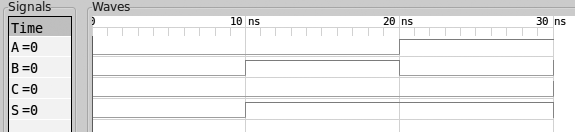
\includegraphics[scale=.4]{images/half-adder-vcd}
	\end{center}
	\caption{The VCD file visualized in the GTKWave Viewer}
	\label{fig:half-adder-gtkwave}
\end{figure}

\section{AUSIM Fault Simulator}
\label{sct:ausim}
% Some discussion on the general use of the simulation
% Capabilities
For the fault simulations performed in this thesis the Auburn University SIMulator or AUSIM\nomenclature{AUSIM}{Auburn University SIMulator} is used.  Developed by Dr. Charles Stroud\cite{ausim}\cite{asl}, AUSIM can perform both logic and fault simulations.  In addition it supports multiple fault models including the gate-level stuck-at and multiple bridging fault models\cite{ausim}.  It supports all of the previously discussed methods of improving simulation time including fault collapsing and parallel fault simulation of both bridging and stuck-at faults\cite{ausim}.  A detailed description of the operation and usage of AUSIM will not be given in this thesis; however, more information can be found in \cite{ausim}\cite{asl}; instead, the focus of this section is an overview of the Auburn Simulation Language or ASL\nomenclature{ASL}{Auburn Simulation Langauge} which is the netlist format used by AUSIM.

\subsection{ASL Netlist Format}
% Format used by AUSIM for simulations
% Discussion of the specifics
Before a circuit can be simulated by AUSIM it must be in a format that AUSIM can understand.  The Auburn Simulation Language (ASL)\nomenclature{ASL}{Auburn Simulation Language} is the circuit description used by AUSIM\cite{asl}.  ASL is used to provide a textual representation of a circuit at the gate-level to the simulator.  This gate-level net-list is used to describe each connection and gate used in a circuit design and allows the simulator to build a representation of the circuit under test.  ASL begins with a top-level circuit declaration.  This declaration defines the name of the circuit and uses the \textit{in} and \textit{out} keywords to define the inputs and outputs to the circuit.  An example circuit is given in Figure \ref{fig:half_adder}.  Figure \ref{fig:half_adder} A is a half-adder which takes in two inputs and outputs a sum and carry bit, the corresponding ASL description is given in Figure \ref{fig:half_adder} B.
\begin{figure}
	\begin{center}
		\begin{minipage}[l]{.45\textwidth}
			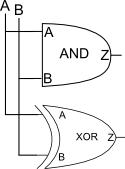
\includegraphics[scale=1]{images/half-adder}	
		\end{minipage}
		\begin{minipage}[r]{.45\textwidth}
			\begin{center}
				Half-Adder Circuit
			\end{center}
			\begin{enumerate}
				\setlength{\itemsep}{0cm}
				\item \# Half-Adder ;
				\item ckt: HF in: A B out: S C ;
				\item xor: X1 in: A B out: S ;
				\item and: A1 in: A B out: C ;
			\end{enumerate}
		\end{minipage}
	\end{center}
	\begin{center}
		\begin{minipage}[l]{.45\textwidth}
			(A)
		\end{minipage}
		\begin{minipage}[r]{.45\textwidth}
			(B)
		\end{minipage}
	\end{center}
	\caption{A Half-Adder circuit}
	\label{fig:half_adder}
\end{figure}
As can be seen from the figure the circuit declaration is started by the \textit{ckt} keyword\cite{asl}.  Each keyword in ASL is followed by a `:' character\cite{asl}.  Following the \textit{ckt} keyword is the name of the circuit in this case ``HF''.  Following that, the primary inputs and outputs are declared using the \textit{in} and \textit{out} keywords.  Each statement in ASL is terminated using a `;' character\cite{asl}.  After the circuit statement the gate-level description of the circuit is given.  The format of each gate is similar to the format of the circuit statement:
\begin{quote}
	\textbf{GATE}: Name \textbf{IN}: In1 In2... InN \textbf{OUT}: Out1 Out2... OutN ;\cite{asl}
\end{quote}
All gate declarations in ASL follow this simple syntax.  All of the elementary logic gates (AND, OR, XOR, etc..) as well as the data flip-flop (DFF)\nomenclature{DFF}{Data Flip-Flop} and two input multiplexer are built-in to AUSIM and available to all circuits\cite{asl}.  Table \ref{tbl:ASLGates} shows each built-in gate and its inputs and outputs.
\begin{table}[bht]
\caption{Built-in AUSIM Gates\cite{asl}}
\begin{center}
\begin{tabular}{|l|l|}
\hline
\multicolumn{2}{|c|}{AUSIM Keywords} \\ \hline
Gate & Example \\ \hline
AND & AND: a1 in: i1.. iN out: Z \\ \hline
OR & OR: o1 in: i1.. iN out: Z \\ \hline
NAND & NAND: na1 in: i1.. iN out: Z \\ \hline
NOR & NOR: no1 in: i1.. iN out: Z \\ \hline
NOT & NOT: n1 in: A out: nA \\ \hline
XOR & XOR: x1: in: i1... iN out: Z \\ \hline
MUX2 & MUX2: m1 in: i1 i2 s1 out: Z \\ \hline
DFF & DFF: d1 in: CLK D out: Q \\ \hline
\end{tabular}
\end{center}
\label{tbl:ASLGates}
\end{table}

It is important to understand that custom gates can be implemented and used in a similar syntax.  To do this one must use the \textit{subckt} command.  While an ASL file can only have a single circuit declaration, it can have any number of sub-circuit declarations\cite{asl}.  Each sub-circuit has its own set of top-level inputs and outputs and its own gate-level net-list.  Once defined the name of the sub-circuit can be used as a gate and be instantiated elsewhere in the circuit description.  These sub-circuit definitions can be used to define the behavior of more complex CMOS gates such as the OAI222 etc.  For the BIST discussed in this thesis, an entire library of sub-circuits was created to support simulation.  This library defines many of the complex CMOS logic gates and several technology specific standard cells.  This library is discussed in more detail in Chapter 3.

\section{BIST Architecture}
% Introduce the bist, its SSA BIST based on a DDS
% some other introductory characteristics

\subsection{Selective Spectrum Analysis}
% Discuss DDS based frequency generation
% Discuss frequency words and how they relate to the clock speed and frequency generation

\subsection{ORA Multiplier-Accumulators}
% Discuss ORA design
% DC1 and DC2 MAC
% Discuss in-phase and out-of-phase accumulations
% Probably will need to briefly mention cordic

\subsection{On-Chip Calculation Circuit}
% Discuss importance of on-chip and how it differs from ORA
% Discuss LOG circuit and how all calculations are performed in log 
% Discuss how calculations are performed for each test and which tests are available
%% Linearity, Frequency Response, Spur Search, SNR, NF

\subsection{Interfacing with BIST}
% Communication mechanism for BIST
% High-level overview of the SPI
% Challenges of testing BIST through SPI?

 
\subsection{Fault Simulation}

\section{BIST Architecture}
Our BIST architecture is a mixed-signal BIST approach which uses Selective Spectrum Analysis (SSA)\nomenclature{SSA}{Selective Spectrum Analysis} to test analog circuitry.  A block diagram of the basic architecture can be seen in Figure \ref{fig:bist-ssa}.  This architecture is capable of measuring a number of different analog characteristics including frequency response and third-order interception point (IP3)\nomenclature{IP3}{Third Order Interception Point}\cite{basessa}.  In addition by sweeping through a frequency spectrum both Signal to Noise Ratio (SNR)\nomenclature{SNR}{Signal to Noise Ratio} and Noise Figure\cite{noisefigure} and be measured.
\begin{figure}
	\begin{center}
		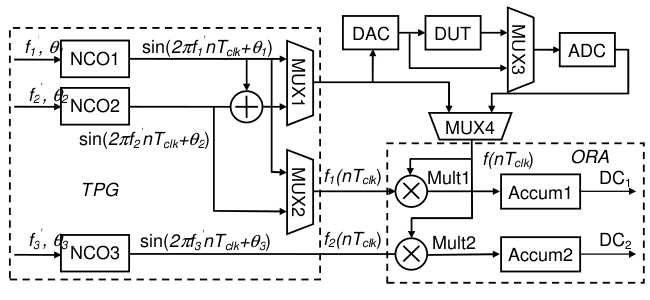
\includegraphics[scale=.5]{images/bist-ssa-architecture}
	\end{center}
	\caption{General BIST Architecture\cite{testtime}}
	\label{fig:bist-ssa}
\end{figure}
As seen in Figure \ref{fig:bist-ssa} the BIST consists of a Direct Digital Synthesis (DDS)\nomenclature{DDS}{Direct Digital Synthesis} based TPG, Multiplier Accumulator (MAC)\nomenclature{MAC}{Multiplier Accumulator} based ORA, and test controller (not shown).  The TPG consists of three numerically controlled oscillators (NCOs)\nomenclature{NCO}{Numerically Controlled Oscillator} and utilizes the existing DAC in the mixed-signal system to generate the analog waveforms for testing\cite{testtime}.  Each NCO has a phase accumulator which is used to generate the output frequency\cite{basessa}.  By accumulating the phase word based on a given frequency word \textit{f} each NCO will generate a frequency according to Equation \ref{eq:frequencyword}\cite{testtime}.  The generated tones serve two purposes: one is to stimulate the analog DUT, and the second is to provide an in-phase and out-of-phase reference tone for the ORA\cite{testtime}
\begin{equation}
	f = \frac{f \times f_{clk}}{2^{n}}
	\label{eq:frequencyword}
\end{equation}

The ORA architecture consists of two MACs.  Each MAC receives the output from the DUT as well either the in-phase or out-of-phase signal from an NCO.  Using this method the ORA is able to measure the amplitude and phase response at a given frequency\cite{testtime}.  Each test the BIST performs relies on this method of measurement.  The tests and how they are run will be discussed in the next section.

In addition to the TPG and MAC-based ORA, there are a number of multiplexers in Figure \ref{fig:bist-ssa}.  These multiplexers define different paths for sending and receiving signal to or from the DUT.  As referenced in Section \ref{sct:MixedSignal} these multiplexed loopback paths can be essential to achieving a high fault coverage when testing.  In the architecture shown there are three loopback paths in the system.  The first path is a path which passes a signal out through MUX1, through the DAC, through the analog DUT and returns it back through the ADC and into MUX4.  This is the outermost path which stimulates the Analog DUT for testing.  A second path exists similar to the first; however, instead of the output of the analog DUT, MUX3 instead selects the bypass path around the DUT.  This bypass path be used to calibrate the BIST for any noise introduced by the DAC and ADC pair.  The final path is the digital loopback path.  In this path MUX4 selects the output from MUX3 directly.  This path bypasses all analog circuitry including the ADC and DAC.  As stated in Section \ref{sct:MixedSignal}, this is the path that is most important for our testing of the BIST.  The digital loopback path does not introduce any analog error into the signal so when performing a ``loopback test'' the test will always result in the same accumulated value, no range of acceptable values is required\cite{stroud-analog}.

\subsection{Performing Tests}
In a single measurement (where a measurement is defined as a single accumulation at a particular frequency) the BIST can measure the magnitude and phase of the DUT output at the measured frequency.  To calculate these values Equation \ref{eq:MagnitudePhase} is applied to the two resulting accumulation values one in-phase and one out-of-phase\cite{jie}.  In the equation DC$_1$ and DC$_2$ are the output of the two in-phase and out-of-phase accumulations.
\begin{equation}
  \begin{tabular}{lll}
	$A(f)$ & $=$ & $\sqrt{DC_1^2+DC_2^2}, \nonumber$ \\
	  $\Delta\phi(f)$ & $=$ & $-\tan^{-1}\frac{DC_2}{DC_1}.$
  \end{tabular}
  \label{eq:MagnitudePhase}
\end{equation}

To perform more complex tests such as frequency response and IP3 (also called linearity) these measurements are performed repeatedly at different frequencies of interest and the results of each tests are used to calculate the result.  As an example during a linearity measurement the DUT is driven by a two-tone signal which consists of two fundamental tones $f_1$ and $f_2$.  Due to the DUT's nonlinearity, its output will consist of not only $f_1$ and $f_2$ but also the third order inter-modulation points (IM3)\nomenclature{IM3}{Third Order Inter-Modulation Point}\cite{testtime}.  Figure \ref{fig:linearity-spectrum} demonstrates what the input and resulting spectrum will look like\cite{testtime}.  The linearity ($\Delta P$) of the DUT can be determined by the difference in dB between the fundamental frequency (either $f_1$ or $f_2$) and the IM3 tone\cite{basessa}.  To calculate this the BIST must take two measurements at either the two lower frequencies $f_1$ and $2*f_1-f_2$ or the two upper frequencies $f_2$ and $2*f_2-f_1$\cite{testtime}.  The result is the difference in the two measured magnitudes.
\begin{figure}
	\begin{center}
		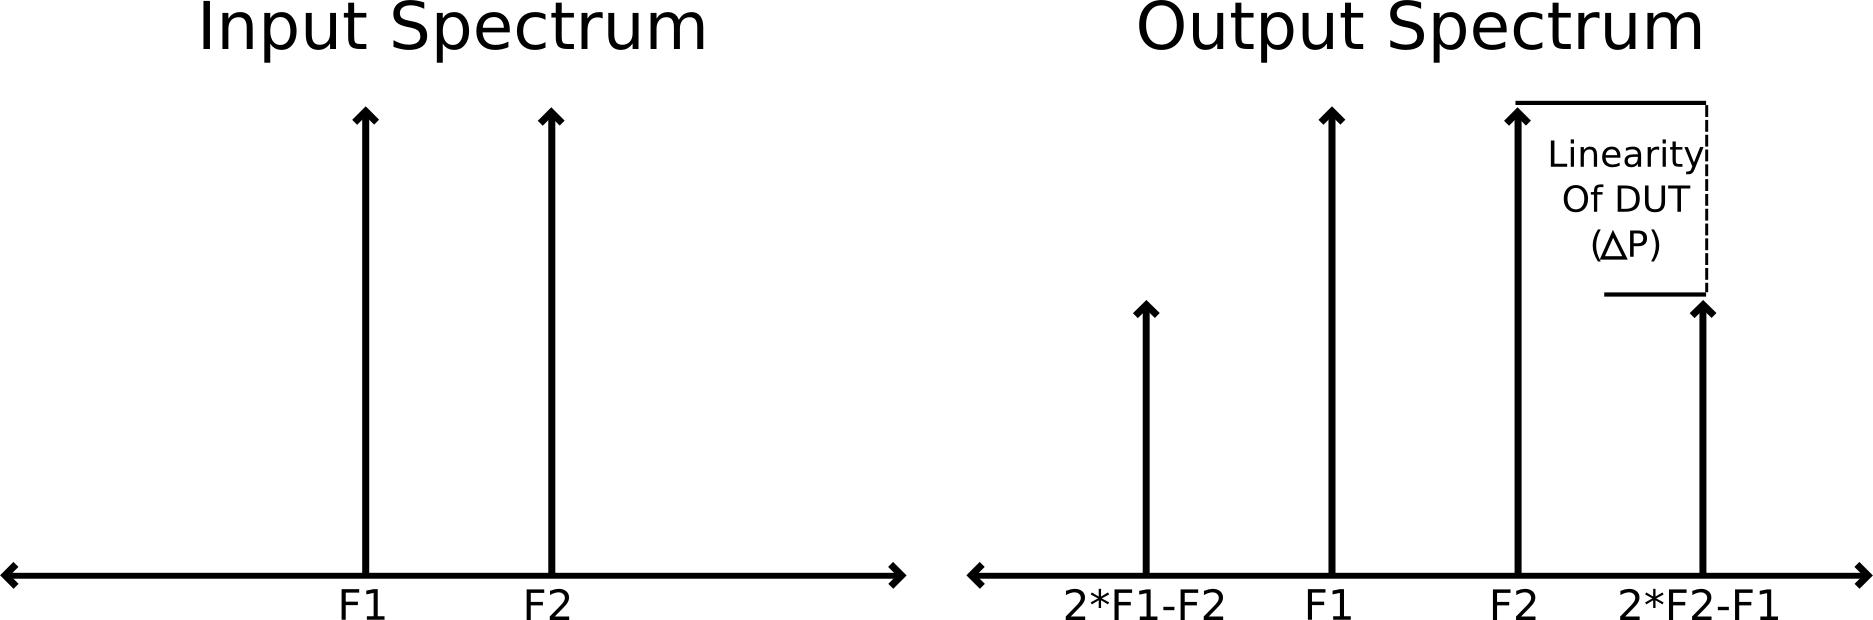
\includegraphics[scale=.7]{images/linearity-spectrum}
	\end{center}
	\caption{Two-tone test for IP3 measurement\cite{testtime}}
	\label{fig:linearity-spectrum}
\end{figure}
The linearity test is just one example of how a measurement is made using this BIST architecture, in the next section more details will be discussed about how calculations are made on-chip and how the test controller is used to control and execute different BIST sequences.  Before discussing the rest of the BIST architecture it is important to understand how the amount of time required for a measurement is determined.  The accumulation is exceptionally important to achieving an accurate measurement due to potential AC calculation errors\cite{jie}.  A large body of work was put into determining both the appropriate length of time to accumulate and a method for determining the length of time efficiently in hardware.  \cite{jie} and \cite{testtime} discuss in detail the complexity of stopping accumulation at the correct moment to reduce the error.  As it is only pertinent to this thesis as it relates to fault simulation time, it will only be briefly discussed here as in relation to test-time.

According to \cite{jie}, there is a potential for calculations errors in an SSA approach.  In an effort to minimize or the errors the BIST approach must either accumulate for a long period of time (referred to as free-run accumulation) or the accumulation time must be stopped at an integer multiple period (IMP)\nomenclature{IMP}{Integer Multiple Period} of the frequency being measured.  As explained in \cite{jie} a good IMP occurs when using a $M_{full}$ width phase accumulator at $2^{M_{eff}}$ accumulation cycles where $M_{eff}$ is calculated in Equation \ref{eq:EffectiveBits}, when m is the bit position of the least significant `1' in a frequency word\cite{jie}.
\begin{equation}
	M_{eff} = M_{full} - m
	\label{eq:EffectiveBits}
\end{equation}
As an example, given a four bit wide phase accumulator and the frequency word 1010 (or decimal 10), $M_{eff}$ would be equal to $4 - 1$ or 3.  This makes the number of clock cycles before a good IMP $2^3$ or $8$.  For large phase accumulators the number of clock cycles to accumulate can vary greatly depending on the frequency word chosen.  In our BIST architecture with 16-bit phase accumulators, the difference between the shortest accumulation time of 2 clock cycles and than the longest accumulation time of 65535 clock cycles (which occurs when using any odd frequency word) is much greater.  Another level of complexity occurs when doing a test which requires more than a single tone.  For a multi-tone test the IMP must be the common IMP of all frequency words.  In practice a simple method is used to determine the common IMP and subsequently the maximum number of clock cycles to accumulate.  By logically OR'ing the frequency words together, our BIST approach uses an OR chain to directly determine the number of clock cycles to accumulate.  Figure \ref{fig:or-chain} shows the or-chain which calculates the number of clock cycles.  The figure easily shows that a logic `1' in the LSB or 0th bit of the input produces a `1' on all the output bits (which corresponds to the maximum number of clock cycles for a given phase accumulator size).
\begin{figure}
	\begin{center}
		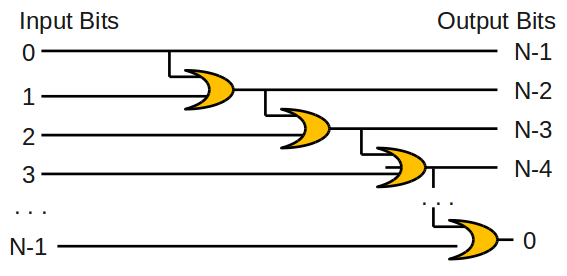
\includegraphics[scale=1]{images/or-chain}
	\end{center}
	\caption{The OR Chain which calculates the number of clock cycles from the logical OR of all frequency words}
	\label{fig:or-chain}
\end{figure}
Using this clock cycle count, the BIST uses a clock cycle counter to determine when to stop accumulation on an IMP and minimize the error.  Once accumulation has completed the calculation step is triggered and the results are handed off the calculation circuit.

\subsection{Calculation Circuitry}
As discussed previously when the BIST is used to measure a frequency, the result is the in-phase and out-of-phase values measured at the given frequency ($DC_1$ and $DC_2$).  While these values contain the magnitude and phase information about the measured frequency, they are in a format which is not intuitive and requires post-processing to determine the result.  To calculate the magnitude and phase the previously discussed equations from Equation \ref{eq:MagnitudePhase} can be used.  While this provides a simple step to converting the $DC_1$ and $DC_2$ values to a more intuitive format, it requires manual post-processing to be completed.  The circuitry that will be discussed brings the processing of the $DC_1$ and $DC_2$ on-chip allowing the magnitude and phase to be determined and output directly.  In addition, with the help of a sophisticated test controller the BIST is capable of taking more complex measurements (such as IM3 and SNR) and produce the output of those higher-order measurements directly.

\cite{joey} discusses the original implementation of the calculation circuitry for our BIST approach.  Shown in Figure \ref{fig:joeycalc} the original calculation circuit uses a custom CORDIC developed by \cite{joey} to perform the operations from Equation \ref{eq:MagnitudePhase} and determine the magnitude and phase from the $DC_1$ and $DC_2$ values.
\begin{figure}
	\begin{center}
		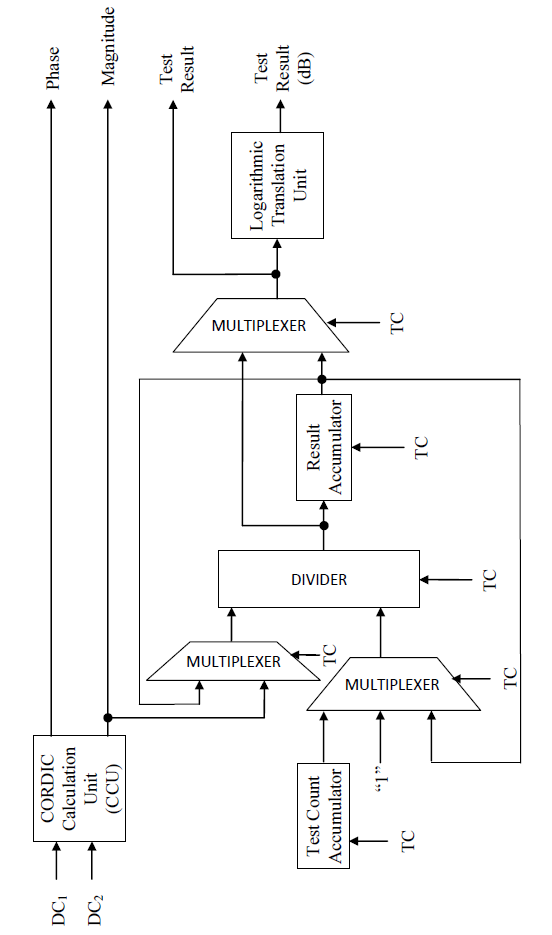
\includegraphics[scale=1]{images/joey-calculation}
	\end{center}
	\caption{Calculation Circuit presented in \cite{joey}}
	\label{fig:joeycalc}
\end{figure}
Also in this circuit is some additional circuitry to perform many of the higher level tests available to the BIST such as the previously discussed IM3 or linearity test.  With the help of the test controller the calculation circuit presented by \cite{joey} can be used for IM3, spur search\footnote{A spur search consists of a measurement from a starting frequency to an ending frequency which returns the frequency and magnitude of the most powerful frequency measured in the given range}, signal-to-noise ratio, and noise figure (NF)\nomenclature{NF}{Noise Figure} tests.  To do this multiple frequency measurements must be made by the BIST and stored in the calculation circuit.  The final result from any such test is converted to decibels by the Logarithmic Translation Unit and made available to the system.  The main feature of the calculation circuit is the divider.  The divider performs several different functions depending on the test.  In a IM3 test the divider is used to divide a current magnitude measurement by a previous measurement; likewise, for the SNR measurement it is used to divide the measured signal magnitude by the summation of the noise in the system\cite{joey}.  The divider and accumulators are also used to find the average noise in the system which is used to calculate the SNR.  While this circuit functions correctly and was able to solve the issue of on-chip calculations there are a number of issues which could be improved.

First the area of the calculation circuit was large, particularly the divider took up a large amount of chip area.  Second the calculation circuit could not run at the same speed as the BIST circuitry.  Our goal for our BIST implementation was to achieve a 1GHz operation frequency.  Unfortunately the calculation circuit could not achieve this speed which necessitated two clock domains one for the BIST which could operate at upto 1GHz and one for the calculation circuit which could operate at upto 500 MHz.  This made the interface circuitry between the BIST and the calculation circuit more complex and error prone.  A third issue which occurred was the potential for divide by zero errors.  Specifically when measuring the noise in the system, divide by zero errors could cause errors in the measurement if the magnitude measured by the BIST was small.

To overcome these problems a new calculation circuit was developed.  Drawing upon the basic operation of the existing circuit the new circuit (Figure \ref{fig:newcalc}) removes the divider in favor of performing all operations in the logarithmic domain.
\begin{figure}
	\begin{center}
		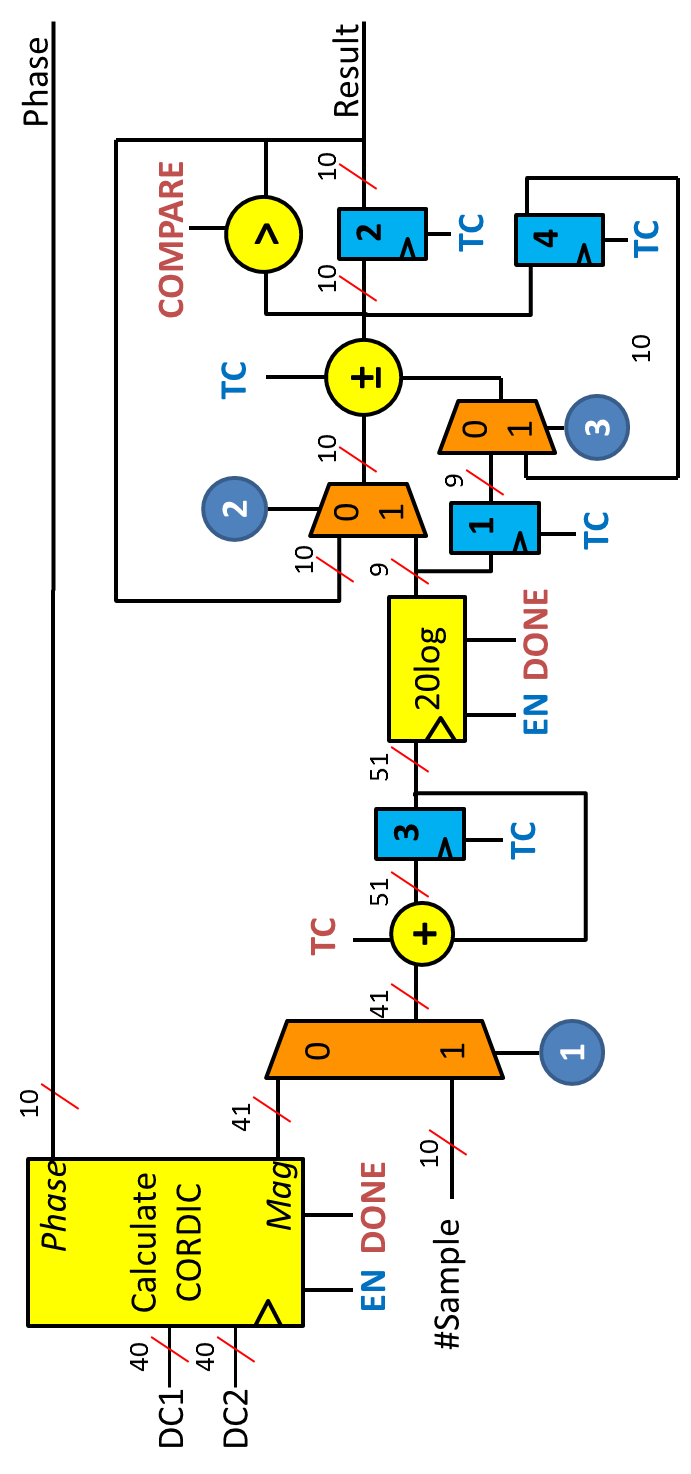
\includegraphics[scale=.8]{images/new-calculation}
	\end{center}
	\caption{New Calculation Circuit}
	\label{fig:newcalc}
\end{figure}
Like the previous calculation circuit it uses a slightly modified calculation CORDIC based on the design by \cite{joey}.  Unlike the previous circuit, the Logarithmic Translation Unit has been moved to the front of the circuit so that all inputs are converted their log value.  This allows for the removal of the divider circuitry as the division required is performed by the subtraction of the two log values.  Consequently, there is no longer an opportunity to perform division by zero since no division operation is occurring.  The new circuit is also able to operate at the same clock frequency as the BIST, eliminating the need for two clock domains.  Finally due to the removal of the divider and other changes in the BIST, the calculation circuit was able to be shrunk to a much smaller size (approximately a 33\% reduction in area and power).

\subsection{Interfacing with the BIST}
Finally given an understanding of the calculation circuit, it is important to be familiar with how our BIST approach is controlled and observed (after all Section \ref{sct:whytest} clearly shows that controllability and observability directly influence the testability of a circuit).  Excluding some run flags, the majority of the BIST is controlled via a SPI interface.  When writing to the SPI interface there is a lower and upper 64-bit word that should be written with the data required for the test being run.  Of the total 128 bits written to the SPI, only 88 of them are actually used by the BIST.  Table \ref{tbl:SPIWrite} shows an overview of the SPI word.  In addition the test control word is broken down in Table \ref{tbl:TestControlWord}.
\begin{table}
	\begin{minipage}[c]{\textwidth}
		\begin{tabular}{|l|l|l|}
			\hline
			Bits & Name & Description \\ \hline
			0-14 & Frequency Word 1 & First frequency of interest\footnote{The frequency words are used in different ways depending on the test being run} \\ \hline
			15-29 & Frequency Word 2 & Second frequency of interest \\ \hline
			30-44 & Frequency Word 3 & Third frequency of interest \\ \hline
			45-59 & Frequency Word 4 & Fourth frequency of interest \\ \hline
			60-69 & Samples & Number of samples to take\footnote{Used for SNR and Spur Search to indicate the number of measurements to take} \\ \hline
			70-85 & Test Control Word & Determines the test to run and how to run it \\ \hline
			86 & Run Force & Makes the BIST run the test after it is loaded \\ \hline
			87 & Disable DDS Disable & Forces the DDS to reset at the start of a test \\ \hline	
		\end{tabular}	
	\end{minipage}
	\caption{SPI Write Command}
	\label{tbl:SPIWrite}
\end{table}
\begin{table}
	\begin{center}
		\begin{tabular}{|l|l|p{4.3in}|}
			\hline
			Bits & Values & Description \\ \hline
			0 & Loopback Path & Allows bypassing the DAC-ADC pair to test the BIST only \\ \hline
			1 & Preset & Allows selection of preset tests* \\ \hline
			2 & Half-IMP & Causes the BIST to wait only half of an IMP length shortening the test time but sacrificing some accuracy \\ \hline
			3 & Noise Floor & Used to select the summation of the noise instead of the SNR result during and SNR test \\ \hline
			4 & Bypass Path & Allows bypassing the DUT to test the DAC-ADC path* \\ \hline		
			6:5 & Test Mode & Select the test to be run \\ \hline
			10:7 & Attenuation & Attenuates the DAC output* \\ \hline
			12:11 & Read & An initial value to be loaded into the register when reading \\ \hline
			13 & Disable DDS & Disables the DDS producing no output \\ \hline
			14 & Disable ORA & Disables the ORA, putting it in reset mode* \\ \hline
			15 & Run Enable & Enables an external run signal* \\ \hline
			& & *Unused during fault simulation \\ \hline
		\end{tabular}
	\end{center}
	\caption{Test Control Word}
	\label{tbl:TestControlWord}
\end{table}

To read data out of the BIST the same SPI is used.  To read data, a write must first occur with the read flag set and must include two address bits.  The address bits are decoded by the test controller and correspond to four different 64-bit words which can be read out of the BIST each containing different calculation data related to the test.  The values retrievable are shown in Table \ref{tbl:readvals}.  In the context of fault simulation it is less important to focus on the values read and instead focus on how many values can be read in relation to the observability of the system.  In the Chapter 3 and Chapter 4 this will be discussed in more detail as it relates to the tests run and potential improvements to the fault coverage by increasing controllability and observability.  
\begin{table}
	\caption{Read Address Values}
	\begin{center}
		\begin{tabular}{|l|l|}
			\hline
			Address & Values \\ \hline
			00 & $DC_1$ \\ \hline
			01 & $DC_2$ \\ \hline
			10 & Magnitude and Phase \\ \hline
			11 & Spur FW, Log Result, Noise Floor Value \\ \hline			
		\end{tabular}
	\end{center}
	\label{tbl:readvals}
\end{table}

In addition to the SPI IO, there are a few other important outputs used in simulation.  First there is the DDS output which is the generated tone for the test being executed, there is also a 10-bit test result output which is updated to the final log value calculated when the test has completed.  Finally, there is a done flag used to denote that the BIST has finished performing the test requested and that the results have been calculated.  

\subsection{Conclusion}
While these descriptions of the BIST are not a comprehensive operating manual, they are provided to give a background of the circuit so that a basic understanding can be developed by the reader.  The focus of the next chapters will shift to the actual fault simulations and away from the underlying architecture except where it relates to potential improvements in fault coverage and the coverage that is achieved.  Overall the goal of the techniques and methods discussed next are to show an effective method to testing mixed-signal built-in self-test systems using our BIST approach both as a benchmark and for context.

\chapter{Fault Simulations}

\subsection{Converting to ASL}
In many cases behavioral models are written in a high-level hardware description language such as VESIC Hardware Description Language (VHDL)\nomenclature{VHDL}{VESIC Hardware Description Language} or Verilog.  These languages allow a behavioral model to be developed of a circuit at a much higher level than ASL's gate-level description.  This means that for large, complex circuits (such as our BIST approach) design in VHDL or Verilog is preferred.  To aid in the simulation of larger circuits a tool was developed to convert a Verilog net-list to an ASL net-list.  This allows a user to write a high-level behavioral description of the circuit, synthesis it down to a Verilog net-list using one of many different CAD tools, then convert it to ASL for fault simulation using the VerilogParser tool.

As a simple example the ISCAS '85 C17 benchmark circuit (Figure \ref{fig:c17_netlist}) was used to demonstrate the conversion process and the differences between a Verilog net-list and an ASL net-list.  In Figure \ref{fig:c17_netlist} A the behavioral model of the C17 circuit has been synthesized into a post-layout net-list in Verilog.  In B the Verilog model has been converted to ASL.
\begin{figure}[t]
	\begin{flushleft}
		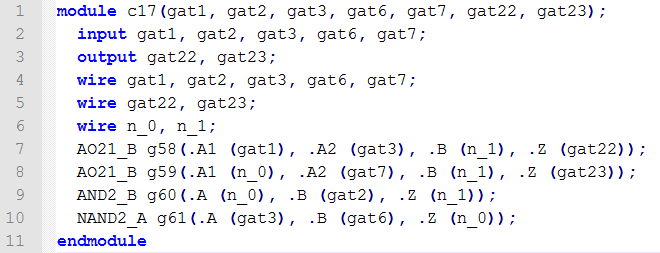
\includegraphics[scale=1]{images/c17-verilog-netlist}	
	\end{flushleft}
	\begin{flushleft}
		(A) Verilog Net-list
	\end{flushleft}
	\begin{flushleft}
		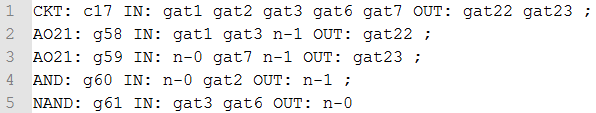
\includegraphics[scale=1]{images/c17-asl-netlist}
	\end{flushleft}
	\begin{flushleft}
		(B) ASL Net-list
	\end{flushleft}
	\caption{C17 Benchmark Circuit Net-list}
	\label{fig:c17_netlist}
\end{figure}
The most significant challenge converting from Verilog to ASL is the difference in the treatment of inputs and outputs of gates and circuits.  In \ref{fig:c17_netlist} A, line 7 the instantiation of the AO21 gate is seen.  The gate's inputs and outputs are not designated separately.  In addition the net names are attached to their respective gate IO names.  In contrast, in \ref{fig:c17_netlist} B, line 2\footnote{The AO21 gate is a custom sub-circuit previously declared} the same gate is instantiated in ASL.  ASL uses a syntax that declares the inputs and outputs to a gate by position and not by name.  For the translation to be successful, the inputs and outputs to the gates must be ordered correctly.  Various techniques including lookup tables must be used to build the ASL correctly.

The VerilogParser tool performs the translation to ASL.  It is written in Microsoft .NET C\# 3.5.  The language was chosen due to the author's familiarity with the language as well as the extensive standard library included in .NET which simplified the program considerably\cite{csharp}.  As a quick reference Figure \ref{fig:VerilogParserUse} demonstrates how to use the tool on a Verilog net-list.
\begin{figure}
	\begin{center}
		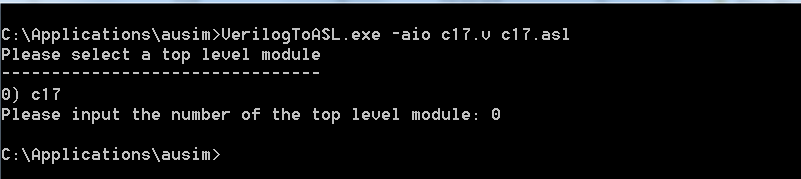
\includegraphics[scale=.9]{images/verilog-asl-command}
	\end{center}
	\caption{Using the Verilog to ASL tool to convert a circuit to ASL}
	\label{fig:VerilogParserUse}
\end{figure}
The tool works by scanning the Verilog file for module definitions and parses the modules into an intermediate representation of the circuit.  It then prompts the user to choose which module should be used as the top-level circuit before outputting the resulting ASL.  Some improvements can be made to the converter such as automatic top-level module detection as well as the ability to convert VHDL net-lists; however, these features were not implemented due to time constraints.  It is important to note that while the ASL generated will always be syntactically correct, the tool does not check for validity of the circuit.  It is assumed any necessary sub-circuits that are used in the net-list have already been created and verified in ASL.  For a more detailed analysis of the Verilog to ASL parser please refer to the Appendix \ref{apdx:VerilogToASL}.  

\subsection{Generating Test Vectors using Vecgen}
Vecgen is a program written to generate AUSIM vector files.  It uses a straight forward command language to build a vector file of any length.  It is written in Microsoft's .NET C\#\cite{csharp} language. Vecgen addresses the issue of large circuits by using a concept called frames.  

The first line of a Vecgen file must be the GENERATE command which tells the generator how many frames(vectors) to generate and the number of primary inputs of the circuit.  If all the user provides is the GENERATE command then Vecgen will create a vector file with the specified number of vectors, filled with all `0' characters as wide as the number of primary inputs in the circuit.  This is the idea behind Vecgen, the vector each time is the same as the vector before it unless changed by the user in a frame.  There are a number of commands which are available to manipulate the output using Vecgen (the full list is available in Appendix \ref{apdx:Vecgen}).  An example generation command file, which would create the vector file shown in Table \ref{tbl:half_adder_vector}, is given in Table \ref{tbl:Vecgen_example} showing the Vecgen format:
\begin{table}
	\label{tbl:Vecgen_example}
	\begin{center}
		\begin{tabular}{l}
			GENERATE 4 2 \\		
			\\
			FRAME 1	\\
			BIT 0 1	\\
			\\
			FRAME 2	\\
			BIT 0 0	\\
			BIT 1 1	\\
			\\
			FRAME 3	\\
			BIT 0 1	\\
		\end{tabular}
	\end{center}
	\caption{Command to generate the half-adder vector sequence}
\end{table}
In the case of the half-adder example, the generator is much more verbose and would not be preferred; however, for this example one can see how it would help in more complex generation.  In our example FRAME 0 is not modified since the first vector generated is always all logic 0's.  FRAME 1 changes bit 0 to a logic 1 so that the resulting vector is now \textit{01}.  FRAME 2 changes bit 0 back to a logic 0 and changes bit 1 to a logic 1, resulting in \textit{10}.  Finally FRAME 3 updates bit 0 back to a logic 1 to obtain the vector \textit{11}.  Only at the times the output vector is changing does a FRAME need to be declared: if we were to generate ten frames instead of the four specified in the example, then the remaining six vectors would be automatically filled in and be the same \textit{11} vector set by FRAME 3.

This is a very simple example, there are many more commands as shown in Appendix \ref{apdx:Vecgen} that allow for much more powerful generation.  Some commands such as RANGE affect multiple bits at once, others such as SERIALIZE or CLOCK work over multiple frames.  One interesting command is the DECLARE command.  The DECLARE command creates a reusable group of commands which can be called from any frame.  This is especially useful if a certain sequence is required repeatedly during a test.  An example sequence and its output are shown in Table \ref{tbl:countsequence}.  The sequence creates a clock on its MSB, then calls a function which counts up then counts back down.  It then disables the clock and calls the counter function again.
\begin{table}
	\caption{Vecgen Example}
	\begin{center}
		\begin{tabular}{l|r|r}
		Commands & 1-15 & 16-24 \\ \hline
		GENERATE 24 3 & 100 & 001 \\
		 & 000 & 000 \\
		\textbf{DECLARE} counter & 101 & 000 \\
		FRAME 0	& 001 & 001 \\
		COUNT 0 2 U & 110 & 001 \\
		FRAME 8 & 010 & 010 \\
		COUNT 0 2 D & 111 & 010 \\
		\textbf{ENDDECLARE} & 011 & 011 \\ 
		 & 100 & 011 \\
 		\textbf{FRAME 0} & 000 & \\
		CLOCK 2 & 111 &  \\
		CALL counter & 011 & \\
		\textbf{FRAME 16} & 110 & \\
		BIT 2 0 & 010 &  \\
		CALL counter & 101 & \\
		\end{tabular}
	\end{center}
	\label{tbl:countsequence}
\end{table}
The generation in Table \ref{tbl:countsequence} is much more powerful than the previous example in Table \ref{tbl:Vecgen_example} and demonstrates some of the power that the Vecgen program provides.  All fault simulation tests for the BIST are designed in the Vecgen markup language for simplicity.

\chapter{Simulation Results}

\chapter{Conclusions and Summary}

% Bibliography
\begin{thebibliography}{99}
\bibitem{stroud} Charles Stroud, {\em A Designer's Guide to Built-In Self-Test}, Vishwani D. Agrawal, Ed. Dordrecht: Kluwer Academic Publishers, 2002.

\bibitem{itrs} ITRS 2009 (I am not sure how to cite this I need to ask you about it)

\bibitem{zorian} Yervant Zorian, "Testing the monster chip," {\em Spectrum, IEEE}, vol. 37, no. 7, pp. 54-60, July 1999.

\bibitem{ungar} Louis Ungar and Tony Ambler, "Economics of Built-In Self-Test," {\em Design \& Test of Computers, IEEE}, vol. 18, no. 5, pp. 70-79, Sep-Oct 2001, \url{http://ieeexplore.ieee.org/stamp/stamp.jsp?tp=&arnumber=953274&isnumber=20606}.

\bibitem{syschip} Laung-Terng Wang, Nur Touba, and Charles Stroud, Eds., {\em System On Chip Test Architectures}. Burlington, MA: Elsevier, 2008.

\bibitem{milor} Linda Milor and V Visvanathan, "Detection of Catastrophic Faults in Analog Integrated Circuits," {\em IEEE Transactions on Computered-Aided Design of Integrated Circuits and Systems}, vol. 8, no. 2, pp. 114-130, Feburary 1989.

\bibitem{stroud-analog} Charles Stroud, Piyumani Karunaratna, and Eugene Bardley, "Digital Components for Built-In Self-Test of Analog Circuits," in {\em 10th ASIC Conference and Exhibit}, Portland, 1997, pp. 47,51.

\bibitem{ausim}  Charles E. Stroud, "AUSIM: Auburn University SIMulator - version 2.0", Dept. of Electrical \& 
Computer Engineering, Auburn University, July 7, 2003

\bibitem{asl} Charles E. Stroud, "ASL: Auburn Simulation Language", Dept. of Electrical \& Computer
Engineering, Auburn University, July 7, 2003.

\bibitem{verilog} "IEEE Standard Hardware Description Language Based on the Verilog(R) Hardware Description Language," IEEE Std 1364-1995 , vol., no., pp.i, 1996 doi: 10.1109/IEEESTD.1996.81542 URL: \url{http://ieeexplore.ieee.org/stamp/stamp.jsp?tp=&arnumber=803556&isnumber=12005}

\bibitem{testtime} Jie Qin; Stroud, C.; Dai, F.; , "Test time of multiplier/accumulator based output response analyzer in built-in analog functional testing," System Theory, 2009. SSST 2009. 41st Southeastern Symposium on , vol., no., pp.363-367, 15-17 March 2009 doi: 10.1109/SSST.2009.4806795 URL: \url{http://ieeexplore.ieee.org/stamp/stamp.jsp?tp=&arnumber=4806795&isnumber=4806773}

\bibitem{noisefigure} Jie Qin; Stroud, C.; Dai, F.; , "Noise Figure Measurement Using Mixed-Signal BIST," Circuits and Systems, 2007. ISCAS 2007. IEEE International Symposium on , vol., no., pp.2180-2183, 27-30 May 2007 doi: 10.1109/ISCAS.2007.378606 URL: \url{http://ieeexplore.ieee.org/stamp/stamp.jsp?tp=&arnumber=4253104&isnumber=4252535}

\bibitem{basessa} F. Dai, C. Stroud, and D. Yang, “Automatic Linearity and Frequency Response Tests with Built-in Pattern Generator and Analyzer,”  IEEE Trans. on VLSI Systems., vol. 14, no. 6, pp. 561-572, 2006.

\bibitem{csharp} Microsoft. The C\# Language. Visual C\# Developer Center. [Online] \url{http://msdn.microsoft.com/en-us/vcsharp/aa336809.aspx}.

\bibitem{jie} Jie Qin, Selective Spectrum Analysis (SSA) and Numerically Controlled Oscillator (NCO) in Mixed-Signal Built-In Self-Test, Doctoral Dissertation, Auburn University, 2010.

\bibitem{joey} Joey's Thesis

\bibitem{analogfaults} Milor, L.; Visvanathan, V.; , "Detection of catastrophic faults in analog integrated circuits," Computer-Aided Design of Integrated Circuits and Systems, IEEE Transactions on , vol.8, no.2, pp.114-130, Feb 1989 doi: 10.1109/43.21830 URL: \url{http://ieeexplore.ieee.org/stamp/stamp.jsp?tp=&arnumber=21830&isnumber=882}

\bibitem{analogosc} Arabi, K., and B. Kaminska, "Oscillation-Test Strategy for Analog and Mixed-Signal Integrated Circuits," Proc. IEEE VLSI Test Symp.,  1996, pp. 476-482.

\bibitem{faultdiagnosis} Yarmolik, V. \em{Fault diagnosis of digital circuits}. John Wiley & Sons, 1990. Print.

\bibitem{analogmixedtest} Vinnakota, Bapiraju. \em{Analog and mixed-signal test}. Prentice Hall, 1998. Print.


\label{Bibliography}
\end{thebibliography}

\appendix
\addcontentsline{toc}{chapter}{Appendices}

\chapter{Verilog To ASL Parser}
\label{apdx:VerilogToASL}
This appendix reviews the Verilog to ASL parser tool in more detail.  The parser is 837 total lines of code, as such only select portions will be reviewed in this appendix.  

TBD, expect ~2-3 pages

\chapter{Vecgen Commands}
\label{apdx:Vecgen}
This appendix provides a list of all commands usable by the Vecgen program to create test vector files for AUSIM.

TBD, expect ~3-4 pages
\end{document}

